\documentclass[12pt]{article}

\usepackage{sbc-template}
\usepackage{graphicx,url}
\usepackage{enumitem}
\usepackage[brazil]{babel} 
%\usepackage[latin1]{inputenc}
\usepackage[utf8x]{inputenc}
\usepackage{multirow}
\usepackage[table]{xcolor}
     
\sloppy

\title{Usando Certificados Digitais OM-BR para proteção de Medidores de Combustível}
% \author{Nome do Autor\inst{1}}
% 
% \address{Endereço Linha 1\\
%   Endereço Linha 2
%   \email{\{email\}@email.do.aut}
% }

\author{
  Wilson S. Melo Jr.\inst{1}, Raphael C. Machado \inst{1}, Bruno Abreu\inst{1},\\ 
  Ruy Ramos\inst{2}, Luiz F. R. C. Carmo\inst{1,3}}
\address{Instituto Nacional de Metrologia, Qualidade e Tecnologia (Inmetro)\\
  Duque de Caxias, RJ -- Brasil
\nextinstitute
  Instituto Nacional de Tecnologia da Informação\\
  Brasília -- Brasil
\nextinstitute
  Universidade Federal do Rio de Janeiro (UFRJ)\\
  Programa de Pós-Graduação em Informática (PPGI) -- Rio de Janeiro, RJ -- Brasil  
\email{\{wsjunior,rcmachado,beabreu,lfrust\}@inmetro.gov.br, ruy@iti.gov.br}
}

\begin{document} 

\maketitle

%\begin{abstract}
%\end{abstract}
     
%\begin{resumo} 
%\end{resumo}

\section{Introdução}
No mundo todo, a metrologia legal tem o desafio de prover à sociedade a confiabilidade de instrumentos de medição usados em diferentes atividades e relações de consumo \cite{RodriguesFilho2015}.
Nos países em desenvolvimento, tal desafio torna-se ainda mais complexo em função do elevado número de fraudes associadas a esses instrumentos.
\cite{RodriguesFilho2016} apontam que, apenas no Brasil, o prejuízo causado à sociedade em função de fraudes em medição é da ordem de U\$ 300 milhões por ano.
Essas fraudes geralmente ocorrem quando uma entidade maliciosa tenta adulterar as respostas fornecidas por um instrumento de medição, obtendo assim vantagens indevidas na comercialização de um determinado bem.

Nesse cenário, os medidores de combustível, vulgarmente conhecidos como \emph{bombas de combustível}, são talvez os instrumentos mais visados em termos de fraudes e adulteração de medidas.
A literatura relata problemas relacionados a estes instrumentos em diferentes países, tais como Brasil \cite{Leitao2014a,Beteto2016}, México \cite{Luchsinger2008} e Nigéria\cite{Rasheed2017}.
A fraude associada à medição de combustível pode ser extremamente lucrativa, e ao mesmo tempo difícil de ser exposta \cite{Leitao2014a,Beteto2016}.
Isso motiva especialmente a ação de vendedores de combustível maliciosos, que deliberadamente adulteram o medidor de combustível em uma categoria de fraude conhecida como "bomba baixa" \cite{Beteto2016}.

Por mais que o Inmetro intensifique esforços na fiscalização dos medidores de combustível, tal tarefa é complexa em virtude do elevado número de equipamentos e da capilaridade de distribuição destes pelo país.
Tais características tornam a fiscalização extremamente custosa e mesmo ineficiente contra mecanismos de fraude que podem ser furtivos e facilmente desabilitados pelo atacante na iminência de uma inspeção.

Em face dessas dificuldades, muitos esforços tem sido feitos no sentido de tornar o medidor de combustível um instrumento mais robusto contra eventuais ataques.
Uma ideia consiste em se propor requisitos de segurança e proteção de software que são expressos em Regulamentos Técnicos Metrológicos (RTMs) \cite{Leitao2014a}.
Tais requisitos, por sua vez, são verificados pelo Inmetro durante as atividades de aprovação de modelo (\textit{type approval})\cite{RodriguesFilho2015}, previstas na Metrologia Legal como um importante processo para se garantir a confiabilidade metrológica de um instrumento de medição.
Nesse escopo, e com base em pesquisas desenvolvidas pelo Inmetro e em conformidade com padrões bem estabelecidos de proteção de instrumentos de medição controlados por software \cite{EuropeanCooperationinLegalMetrologyWELMEC2015,InternationalOrganizationofLegalMetrologyOIML2008}, o Inmetro propôs a inclusão de dois requisitos essenciais para se garantir a integridade, autenticidade e não repúdio de uma medição:

\begin{itemize}
    \item O uso de assinatura digital do registro legalmente relevante do instrumento, no momento mais próximo possível da concretização de uma medição, e;
    \item O uso de certificados digitais padrão ICP-Brasil, que são aqueles em conformidade com a Infraestrutura de Chave Pública oficial do país.
\end{itemize}

Neste artigo, são descritos de forma detalhada como cada um dos requisitos contribui para a proteção das medições realizados por um medidor de combustível.
Inicialmente, apresenta-se uma visão geral do funcionamento de uma bomba de combustível, e como um de seus componentes, o \textit{pulser}, pode ser construído como um elemento seguro que fornece apenas valores de medição devidamente assinados.
Em seguida, discute-se a adoção de certificados digitais específicos para dispositivos de medição, e como os mesmos agregam confiabilidade ao processo de medição como um todo, tornando-se uma ferramenta de apoio às atividades da metrologia legal.

\section{Trabalhos relacionados}
\subsection{Preliminares}
A assinatura digital constitui uma das principais aplicações da criptografia de chave pública, ou criptografia assimétrica.
Ela se caracteriza por garantir autenticidade, integridade e irrefutabilidade (não repúdio) de uma dada informação.
A autenticidade deriva imediatamente do uso do par de chaves assimétricas. 
Isso porque qualquer informação verificável por meio de uma chave pública tem sua origem intrinsicamente ligada à entidade que possui a respectiva chave privada, permindo assim a identificação e autenticação desta entidade.
A integridade, por sua vez, é obtida por meio da encriptação de um resumo criptográfico da informação.
Por fim, a irrefutabilidade depende do uso de um certificado digital, que nada mais é do que a atestação por uma terceira parte confiável de que determinada chave pública pertence à respectiva entidade.

Autenticidade e integridade estão diretamente ligadas com o simples uso de um algoritmo de criptografia de chave pública e um algoritmo de hash.
A irrefutabilidade, por sua vez, depende de uma infraestrutura de gestão de certificados digitais, também conhecida como Infraestrutura de Chave Pública (ICP).
No contexto de uma ICP, três papéis são de fundamental importância para se garantir o devido funcionamento de sistemas baseados em assinaturas digitais:

\begin{itemize}
    \item Autoridade Certificadora (AC): é a autoridade responsável pela emissão, distribuição, renovação, revogação e gerenciamento dos certificados digitais. Na prática, a AC é responsável por assinar os certificados digitais com sua própria chave privada, atestando assim a correspondência destes às suas respectivas entidades.
    \item Autoridade de Registro (AR): é a autoridade responsável pela interface entre a AC e entidade interessada em ter um certificado digital (usuário). A AR tem a função de receber, validar e encaminhar solicitações de um usuário para a AC.
    \item Autoridade Certificadora Raiz (AC-Raiz): é a primeira autoridade da cadeia de certificação, responsável por fiscalizar e auditar outras ACs e ARs. Sendo ela mesma uma AC, é também responsável pela  emissão, distribuição, renovação, revogação e gerenciamento dos certificados digitais das demais ACs. No Brasil, esse papel compete ao Instituto de Tecnologia da Informação (ITI);
\end{itemize}

\subsection{Assinatura digital em instrumentos de medição}
Embora o uso de assinatura digital, bem como de certificados digitais, seja um tema amplamente consolidado no contexto de segurança da informação, o mesmo constitui uma prática relativamente recente em aplicações envolvendo instrumentos de medição.

Trabalhos correlatos são encontrados em aplicações diversas envolvendo sensores e dispositivos IoT (Internet of Things) \cite{Jing2014,Ray2015,AlSalami2016}.
O uso de criptografia de chave pública e também de certificados digitais é amplamente difundido em soluções de segurança para tais aplicações.
Tal abordagem é justificada pelo simples fato de tentar se aplicar um modelo extremamente consolidado em outros cenários envolvendo redes e sistemas computacionais.
Todavia, existem também aspectos negativos a serem considerados.
A complexidade inerente à manutenção de uma ICP, bem como os custo computacional associado ao uso de algoritmos criptográficos, justifica o reaproveitamento de infraestruturas já existentes \cite{Ray2015} ou ainda a implementação de soluções de certificação digital simplificadas \cite{AlSalami2016}, visando a redução do custo computacional em dispositivos que apresentam restrições nesse quesito.

Por sua vez, o uso de tal tecnologia em instrumentos de medição ainda é escasso.
Os guias de diretivas de proteção sofware de instrumentos de medição WELMEC 7.2 \cite{EuropeanCooperationinLegalMetrologyWELMEC2015} a OIML D 31 \cite{InternationalOrganizationofLegalMetrologyOIML2008} fazem menção ao conceito de \emph{assinatura de chave pública}, argumentando que chaves assimétricas podem ser usadas para prover autenticidade e integridade dos registros legalmente relevantes de um instrumento.
Todavia, esses guias não fazem qualquer menção ao uso de certificados digitais.


\section{Como funciona uma bomba de combustível}
Um medidor de combustível basicamente bombeia o combustível de um tanque subterrâneo, passando por um transdutor de medição responsável pela medição.
O combustível segue então por um duto ou mangueira, sob o controle de uma válvula solenóide, sendo por fim injetado por meio de um bico no tanque do carro.
O transdutor é tipicamente representado por um eixo mecânico integrado a um pulsador.
O movimento do eixo é convertido em pulsos eletrônicos, de modo que o número de pulsos é proporcional ao volume medido.
Em função disso, o conjunto mecânico que inclui o transdutor é denominado \textit{pulser}.
A Figura \ref{f:transducer} ilustra o funcionamento do \textit{pulser} em um típico modelo de medidor de combustível.

\begin{figure}[ht]
\centering
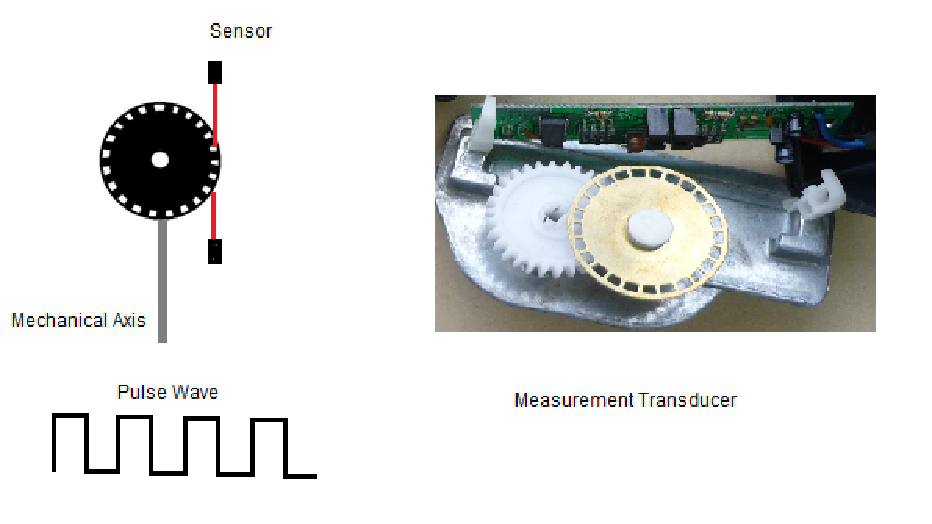
\includegraphics[width=0.9\textwidth]{transducer}
\caption{Princípio de funcionamento de um medidor de combustível}
\label{f:transducer}
\end{figure}

\section{Principais ataques em medidores de combustível}
A norma técnica NIT-Sinst-022 documenta diferentes tipos de ataques contra bombas de combustível detectados e catalogados por agentes do Inmetro no período de 2013 a 2016.
Entre os principais ataques é possível citar:

\subsection{Fraudes em placas controladoras do \textit{pulser}}


\subsection{Fraudes em placas controladoras do \textit{pulser}}
São os casos onde componentes eletrônicos associados à placa de contagem de pulsos são modificados (ou inseridos) de modo a incrementar o número de pulsos, resultando assim em uma medição fraudulenta.


\subsection{Fraudes usando sistemas de gerenciamento}
Essa categoria de fraude caracteriza-se pelo uso de um mecanismo de ataque baseado na ideia de \textit{man-in-the-middle}.
Para tanto ele se vale do sistema de gerenciamento do medidor de combustível.
Esse sistema é externo ao medidor e tem a função de obter informações e enviar comandos específicos.
Quando fraudado, o sistema de gerenciamento é programado para interceptar a informação de medição dada pelo \textit{pulser}, modificá-la acrescentando um valor maior e retornar esse valor adulterado ao medidor de combustível, para que o mesmo seja exibido no \textit{display} disponibilizado ao consumidor.


\section{Uso de certificados digitais}
Esboço feito pelo Raphael sobre o processo:

\subsection{Fabricação do Pulser}
Neste novo modelo de medidor de combustível, o pulser é concebido como um dispositivo único e selado.
Isso implica que todos os subcomponentes responsáveis por suas funcionalidades são encapsulados em um invólucro de segurança.
Em caso de defeito em qualquer dos seus subcomponentes, o pulser deve ser substituído como um todo.
Não existe a possibilidade de reparos funcionais envolvendo a substituição ou reparação de subcomponentes do pulser.

Além dos subcomponentes diretamente associados à eletrônica responsável pela medição de combustível, o pulser inclui também um módulo criptográfico OM-BR.
Deste modo, cada pulser possui seu próprio par de chaves assimétricas, atribuídas de forma única.
O módulo criptográfico permite a divulgação da chave pública do pulser, ao passo que a chave privada é permanentemente protegida pelo módulo criptográfica, sem ser jamais revelada pelo mesmo.
Uma vez que o próprio pulser isola seus subcomponentes por meio do invólucro de segurança, o mesmo protege o módulo criptográfico inclusive contra ataques \textit{side channel}.

Cada pulser é associado a um identificador único, correspondente a seu número de série.
A chave pública do pulser também pode constituir um identificador, dado seu caráter único.
Deste modo, pode-se dizer que existem dois identificadores, um forte e um fraco, sendo esses respectivamente a chave pública do pulser e seu número de série.

\subsection{Fabricação do medidor de combustível}
A fabricação do medidor de combustível envolve a integração do pulser aos demais componentes de constituição mecânica, hidráulica, elétrica e eletrônica que o constituem.
É importante observar, todavia, que o pulser passa a incorporar todas as funcionalidades legalmente relevantes do medidor.
Ainda que outros componentes sejam usados para exibição de informação legalmente relevante (e.g., \textit{display} informando o volume abastecido em litros), tal informação é rastreável à assinatura digital da medição feita pelo pulser, o que encerra a cadeia legalmente relevante.

O medidor como um todo possui também um número de série, atribuido pelo fabricante como um mecanismo de controle de produção.
Quando o pulser é instalado no medidor de combustível, o fabricante associa o identificador do pulser ao respectivo número de série do medidor.
É importante observar que essa associação existe enquanto o pulser se encontra funcional dentro deste medidor.
Se em algum momento a substituição do pulser se faz necessária, essa associação é atualizada, de modo a se manter o controle de qual pulser se encontra funcional dentro de cada medidor de combustível.

\subsection{Verificação inicial}
A verificação inicial é feita por um organismo de inspeção delegado pela autoridade regulamentadora em cada novo medidor de combustível.
A mesma ocorre ainda em fábrica, constituindo um pré-requisito para a comercialização do mesmo.
Nessa verificação, o organismo de inspeção verifica se o instrumento apresenta as características de projeto correspondentes à sua aprovação de modelo, bem como executa testes metrológicos para se certificar de que a incerteza de medição apresentada pelo instrumento se encontra dentro dos limites aceitáveis.
Em seguida, o organismo de inspeção exerce também a atividade de Autoridade de Registro, verificando a existência da chave pública do medidor (e sua correspondente chave privada), bem como coletando as informações de cunho legal que comporão o certificado digital OM-BR deste medidor.
Consequentemente, o organismo de inspeção torna-se também o responsável pela emissão das informações à respectiva Autoridade Certificadora.

\subsection{Emissão do certificado digital}
De posse das informações ja verificadas pela AR, a AC é responsável pela emissão do certificado digital OM-BR a ser embarcado no medidor de combustível.
Como já discutido anteriormente, o certificado digital associa de forma única e irrefutável o respectivo medidor de combustível a sua chave pública.
Desta forma, as medições obtidas a partir deste instrumento de medição tem sua rastreabilidade assegurada, sendo impossível a negação de que determinada medição não foi gerada pelo respectivo pulser.

Uma vez gerado o certificado digital, o mesmo é remetido ao fabricante, para que este proceda com a gravação do mesmo no respectivo instrumento.
A possibilidade de que o fabricante não proceda com a gravação do certificado, ou ainda que a gravação do certificado seja feita em um medidor de combustivel distinto, são irrevalentes.
Isso porque, na incidência de qualquer uma das situações, o medidor será incapaz de realizar suas funções de forma apropriada.
Deste modo, tais situações são detectadas de imedito na operação do instrumento.

\subsection{Instalação em campo}
Uma vez concluidas as etapas anteriores, o medidor de combustível pode ser comercializado e instalado em campo normalmente.
As oficinas autorizadas responsáveis por essa tarefa ficam também responsáveis por informar ao organismo de inspeção o identificador do medidor, identificador do seu respectivo pulser no momento da instalação, bem como o local de instalação do mesmo e as informações relevantes do detentar do instrumento (e.g., CNPJ e razão social do posto de combustível).

Periodicamente, o organismo de inspeção realiza a verificação do medidor em seu respectivo local de operação.
Nessas circunstâncias, além de proceder com a verificação das funcionalidades metrológica e legalmente relevantes, o organismo de inspeção confirma também se a respectiva associação entre o identificador do medidor, o identificador do pulser e as informações complementares do detentor do instrumento permanecem consistentes.
Tal procedimento garante que não ocorreram substituições indevidas do pulser, ou ainda a realocação do medidor de combustível como um todo.

\subsection{Substituição de pulser e realocações de medidores de combustível}
Em caso de necessidade de substituição de um pulser, seja por defeito ou violação do mesmo, ou ainda de realocação do medidor de combustível como um todo para um novo ponto de instalação, a oficina autorizada responsável deve comunicar o evento ao organismo de inspeção, procedendo conforme definido na subseção anterior.

\begin{figure}[ht]
\centering
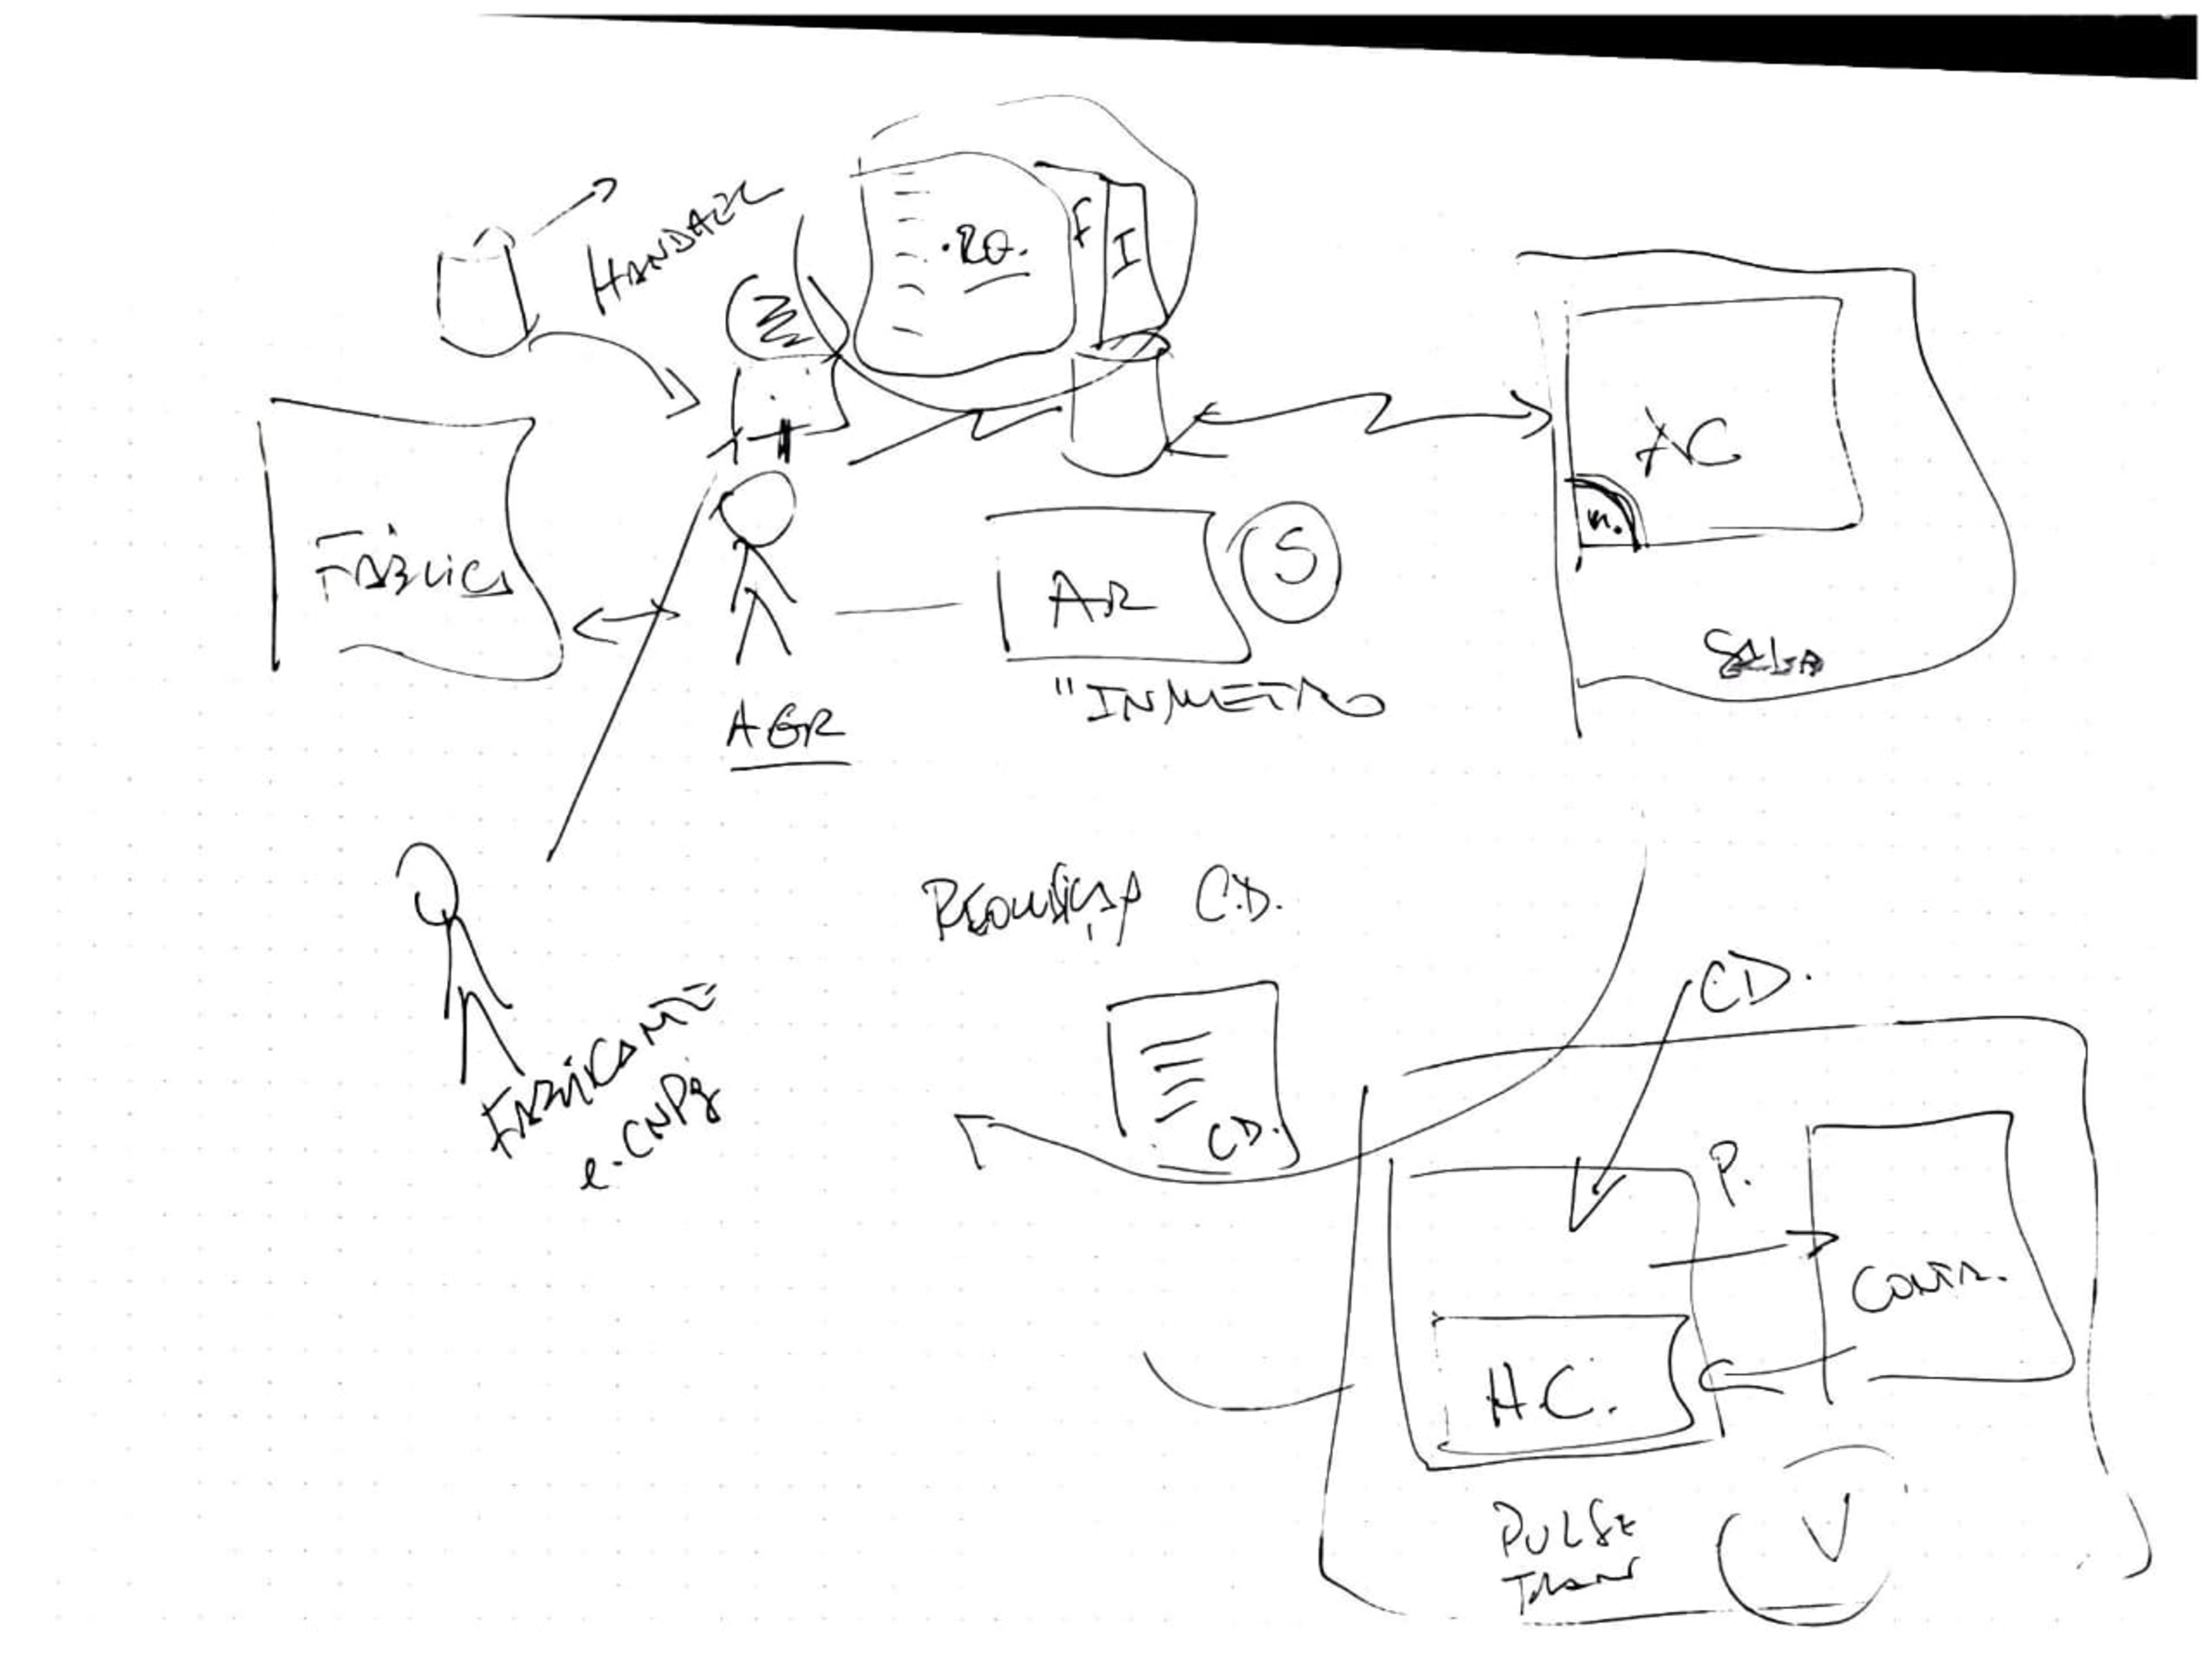
\includegraphics[width=1\textwidth]{ruy.pdf}
\caption{Diagrama descrevendo papéis de AR e AC}
\label{f:ruy}
\end{figure}

%\pagebreak

% Figure and table captions should be centered if less than one line
% (Figure~\ref{fig:exampleFig1}), otherwise justified and indented by 0.8cm on
% both margins, as shown in Figure~\ref{fig:exampleFig2}. The caption font must
% be Helvetica, 10 point, boldface, with 6 points of space before and after each
% caption.
% 
% \begin{figure}[ht]
% \centering
% \includegraphics[width=.5\textwidth]{fig1.jpg}
% \caption{A typical figure}
% \label{fig:exampleFig1}
% \end{figure}
% 
% \begin{figure}[ht]
% \centering
% \includegraphics[width=.3\textwidth]{fig2.jpg}
% \caption{This figure is an example of a figure caption taking more than one
%   line and justified considering margins mentioned in Section~\ref{sec:figs}.}
% \label{fig:exampleFig2}
% \end{figure}
% 
% In tables, try to avoid the use of colored or shaded backgrounds, and avoid
% thick, doubled, or unnecessary framing lines. When reporting empirical data,
% do not use more decimal digits than warranted by their precision and
% reproducibility. Table caption must be placed before the table (see Table 1)
% and the font used must also be Helvetica, 10 point, boldface, with 6 points of
% space before and after each caption.
% 
% \begin{table}[ht]
% \centering
% \caption{Variables to be considered on the evaluation of interaction
%   techniques}
% \label{tab:exTable1}
% \includegraphics[width=.7\textwidth]{table.jpg}
% \end{table}

\bibliographystyle{sbc}
\bibliography{icp-om}

\end{document}
